\chapter{Om Kojo}
\begin{multicols}{2}
\section*{\color{black}Vad är Kojo?}
Kojo är en app som hjälper dig att lära dig att programmera. Med Kojo kan du koda i det moderna och kraftfulla programspråket {\bf\color{blue}Scala}. Kojo är gratis och finns på Svenska. Kojo fungerar med Linux, Windows och Mac OSX.
\section*{\color{black}Var hittar jag Kojo?}
Ladda ner Kojo här: 
\\

\href{http://www.kogics.net/kojo-download}{www.kogics.net/kojo-download}
\\

Läs mer här: 
\\

\href{http://lth.se/programmera}{lth.se/programmera}

\columnbreak

\begin{center}
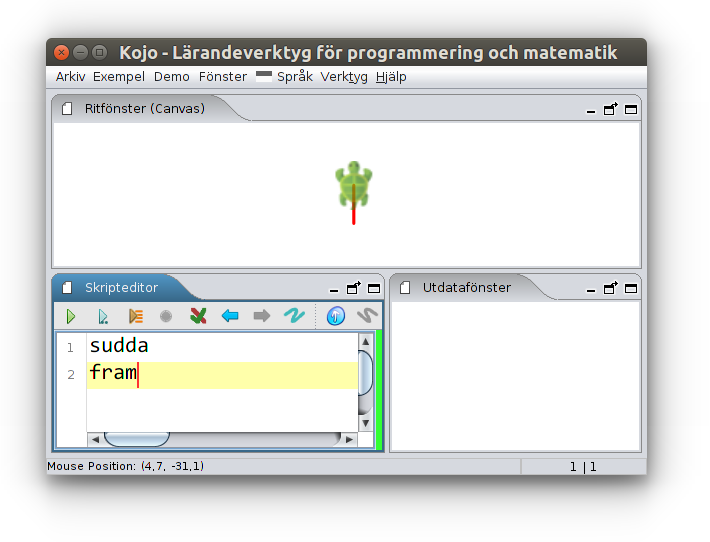
\includegraphics[width=14.0cm]{../img/kojo.png}
\end{center}

\end{multicols}

\chapter{Ditt första program}
\begin{multicols}{2}
\section*{\color{BrickRed}Uppdrag:}
Skriv så här i Kojos skripteditor-fönster:

\begin{lstlisting}[basicstyle={\ttfamily\fontsize{48}{58}\selectfont},numbers=none]
sudda
fram
\end{lstlisting}
        
Tryck på den gröna play-knappen 

\includegraphics[width=1.0cm]{../img/play.png}
\\

för att köra igång ditt program.

\columnbreak

\begin{center}
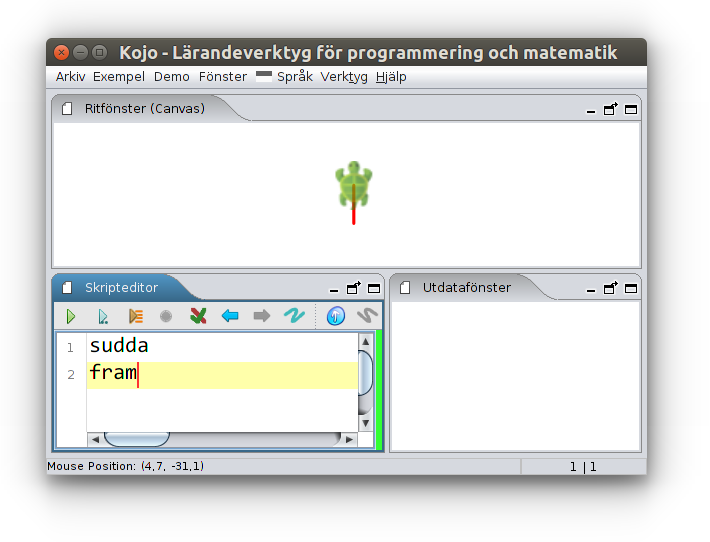
\includegraphics[width=14.0cm]{../img/fram.png}
\end{center}

\end{multicols}

\chapter{Rita en kvadrat}
\begin{multicols}{2}

\begin{lstlisting}[basicstyle={\ttfamily\fontsize{36}{43}\selectfont},numbers=none]
sudda
fram
höger
\end{lstlisting}
        
Om du skriver \lstinline{vänster} eller \lstinline{höger} så vrider sig paddan.
\section*{\color{BrickRed}Uppdrag:}
Utöka programmet så att det blir en kvadrat.

\columnbreak

\begin{center}
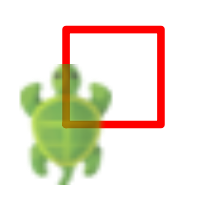
\includegraphics{../img/square.png}
\end{center}

\end{multicols}

\chapter{Rita en trappa}
\begin{multicols}{2}

\begin{lstlisting}[basicstyle={\ttfamily\fontsize{36}{43}\selectfont},numbers=none]
sudda
fram; vänster
fram; höger
\end{lstlisting}
        
\vskip 1.0em
Med semikolon \lstinline{;} kan du ha flera satser på samma rad.
\section*{\color{BrickRed}Uppdrag:}
Utöka programmet så att det blir en trappa.

\columnbreak

\begin{center}
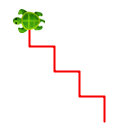
\includegraphics{../img/stairs.png}
\end{center}

\end{multicols}

\chapter{Gör en loop}
\begin{multicols}{2}

\begin{lstlisting}[basicstyle={\ttfamily\fontsize{36}{43}\selectfont},numbers=none]
sudda
upprepa(4){ fram; höger }
\end{lstlisting}
        
\section*{\color{BrickRed}Uppdrag:}


\begin{itemize}

\item {Vad händer om du ändrar 4 till 100?}
\item {Rita en trappa med 100 trappsteg.}

\end{itemize}



\columnbreak

\begin{center}
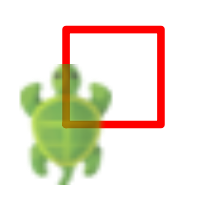
\includegraphics{../img/square.png}
\end{center}

\end{multicols}

\chapter{Rita en gubbe}
\begin{multicols}{2}
\section*{\color{BrickRed}Uppdrag:}
Rita en gubbe som du själv vill.
\section*{\color{OliveGreen}Tips:}

\begin{lstlisting}[basicstyle={\ttfamily\fontsize{24}{29}\selectfont},numbers=none]
hoppa
vänster(180)
fram(300)
hoppa(100)
hoppaTill(25,-28)
skriv("FELIX är bäst")
\end{lstlisting}
        
Du kan se paddans läge nere till vänster medan du rör muspekaren i Ritfönstret:
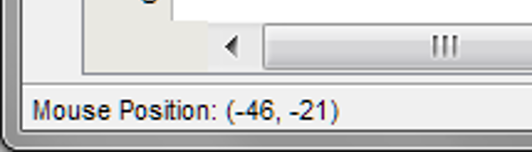
\includegraphics[width=6.0cm]{../img/mousepos.png}


\columnbreak


\begin{center}
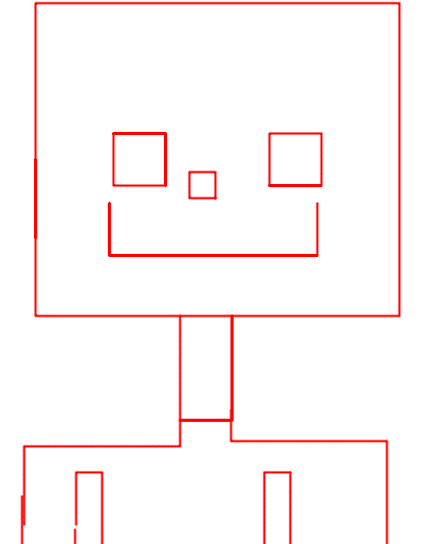
\includegraphics[width=4.5cm]{../img/man.png}
\end{center}

\vskip 2.0em
\begin{center}
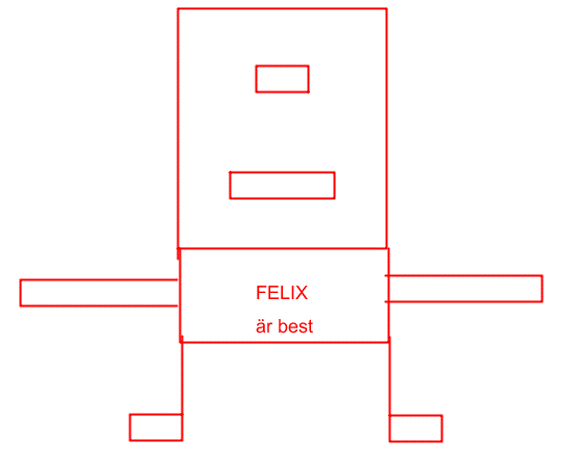
\includegraphics[width=9.0cm]{../img/alien.png}
\end{center}

\end{multicols}

\chapter{Gör din egen funktion}Med \lstinline{def} kan du göra egna {\it funktioner} som du själv väljer namn på.

\begin{lstlisting}[basicstyle={\ttfamily\fontsize{20}{24}\selectfont},numbers=none]
def kvadrat =  upprepa(4){ fram; höger }  

sudda
kvadrat    //använd din kvadrat-funktion
hoppa
kvadrat
\end{lstlisting}
        
\section*{\color{BrickRed}Uppdrag:}


\begin{itemize}

\item {Byt färg på kvadraterna.}
\item {Gör fler kvadrater.}

\end{itemize}


\section*{\color{OliveGreen}Tips:}

\begin{lstlisting}[numbers=none]
fyll(grön); färg(lila)
\end{lstlisting}
        
\chapter{Stapla kvadrater}
\begin{multicols}{2}
\section*{\color{BrickRed}Uppdrag:}
Gör en stapel med 10 kvadrater.
\section*{\color{OliveGreen}Tips:}
\vskip 1.0em

\begin{lstlisting}[numbers=none]
def kvadrat =  upprepa(4){ fram; höger }  

sudda; sakta(100)
upprepa(10){ ??? }
\end{lstlisting}
        

\columnbreak

\begin{center}
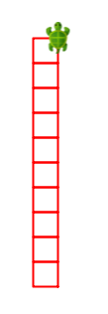
\includegraphics{../img/square-column.png}
\end{center}

\end{multicols}

\chapter{Gör en stapelfunktion}
\begin{multicols}{2}
\section*{\color{BrickRed}Uppdrag:}
Gör en funktion som heter \lstinline{stapel}, som ritar en stapel med 10 kvadrater.
\section*{\color{OliveGreen}Tips:}

\begin{lstlisting}[numbers=none]
def kvadrat = upprepa(4){ fram; höger }  
def stapel = ???

sudda; sakta(100)
stapel
\end{lstlisting}
        

\columnbreak

\begin{center}
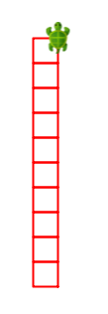
\includegraphics{../img/square-column.png}
\end{center}

\end{multicols}

\chapter{Gör ett rutnät}
\begin{multicols}{2}
\section*{\color{BrickRed}Uppdrag:}
Gör ett rutnät med 10*10 kvadrater.
\section*{\color{OliveGreen}Tips:}


\begin{itemize}

\item {Använd din stapelfunktion från tidigare.}
\item {Du kan hoppa baklänges en hel stapelhöjd med \lstinline{hoppa(-10*25)}}
\item {Du kan sedan hoppa till rätt plats med \lstinline{höger; hoppa; vänster}}

\end{itemize}



\columnbreak

\begin{center}
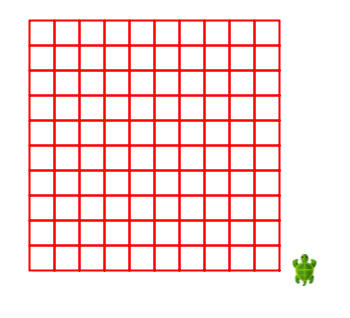
\includegraphics{../img/square-grid.png}
\end{center}

\end{multicols}

\chapter{Kvadrat med parameter}
\begin{multicols}{2}
\section*{\color{BrickRed}Uppdrag:}
Rita olika stora kvadrater.
\section*{\color{OliveGreen}Tips:}
Ge din kvadrat-funktion en {\it parameter},\\
med namnet \lstinline{sidlängd} och typen \lstinline{Heltal}:

\begin{lstlisting}[basicstyle={\ttfamily\fontsize{16}{19}\selectfont},numbers=none]
def kvadrat(sidlängd : Heltal) = 
  upprepa(4){ fram(sidlängd); höger }

sudda; sakta(100); osynlig
kvadrat(100) 
kvadrat(70)
kvadrat(40)
\end{lstlisting}
        
Du kan byta färg med:\\
\lstinline{fyll(blå); färg(rosa)}


\columnbreak


\begin{center}
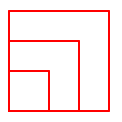
\includegraphics[width=5.0cm]{../img/square-param.png}
\end{center}

\begin{center}
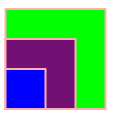
\includegraphics[width=5.0cm]{../img/square-param-color.png}
\end{center}

\end{multicols}

\chapter{Rita en kvadratgubbe}\section*{\color{BrickRed}Uppdrag:}
Rita en gubbe med hjälp av olika stora kvadrater.
\\


\begin{tikzpicture}[overlay]
\node at (20.0cm,0.5cm) {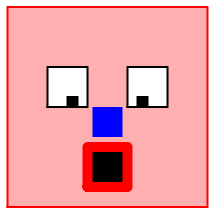
\includegraphics[width=5.5cm]{../img/square-man.png}};
\end{tikzpicture}
  
\section*{\color{OliveGreen}Tips:}

\begin{lstlisting}[basicstyle={\ttfamily\fontsize{14}{17}\selectfont},numbers=none]
def kvadrat(x: Heltal, y: Heltal, sidlängd: Heltal) = {
  hoppaTill(x, y)
  upprepa(4) { fram(sidlängd); höger }
}
def huvud(x: Heltal, y: Heltal) = { fyll(rosa); färg(röd); kvadrat(x, y, 200) }
def öga(x: Heltal, y: Heltal) = { fyll(vit); färg(svart); kvadrat(x, y, 40) }
def pupill(x: Heltal, y: Heltal) = { fyll(svart); färg(svart); kvadrat(x, y, 10) }
def näsa(x: Heltal, y: Heltal) = { fyll(blå); färg(genomskinlig); kvadrat(x, y, 30) }
def mun(x: Heltal, y: Heltal) = { bredd(10); fyll(svart); färg(röd); kvadrat(x, y, 40) }

sudda; sakta(20); osynlig
huvud(0, 0)
öga(40, 100); pupill(60, 100)
???
\end{lstlisting}
        
\chapter{Rita en polygon}\section*{\color{BrickRed}Uppdrag:}


\begin{itemize}

\item {Prova koden nedan. Rita olika slags polygoner.}
\item {Lägg till en parameter \lstinline{sidlängd} och rita olika stora polygoner.}
\item {Hur stort behöver n vara för att det ska se ut som en cirkel?}

\end{itemize}


\section*{\color{OliveGreen}Tips:}

\begin{lstlisting}[basicstyle={\ttfamily\fontsize{18}{22}\selectfont},numbers=none]
def polygon(n:Heltal) = upprepa(n){
  fram(100)
  vänster(360.0/n)
}

sudda; sakta(100)
polygon(7)
\end{lstlisting}
        

\begin{tikzpicture}[overlay]
\node at (20.0cm,3.5cm) {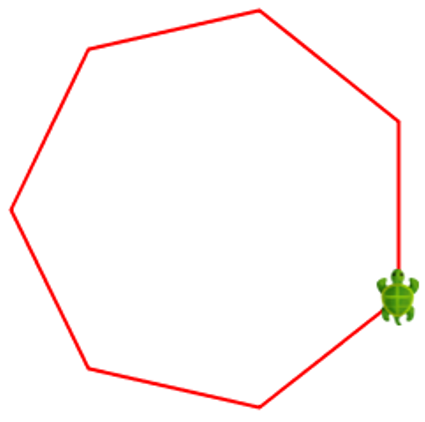
\includegraphics[width=8.0cm]{../img/polygon.png}};
\end{tikzpicture}
  
\chapter{Rita många polygoner}\section*{\color{BrickRed}Uppdrag:}


\begin{itemize}

\item {Prova programmet nedan.}
\item {Prova ändra antalet sidor och vinkel.}
\item {Fyll polygonerna med färg.}

\end{itemize}



\begin{tikzpicture}[overlay]
\node at (21.0cm,1.0cm) {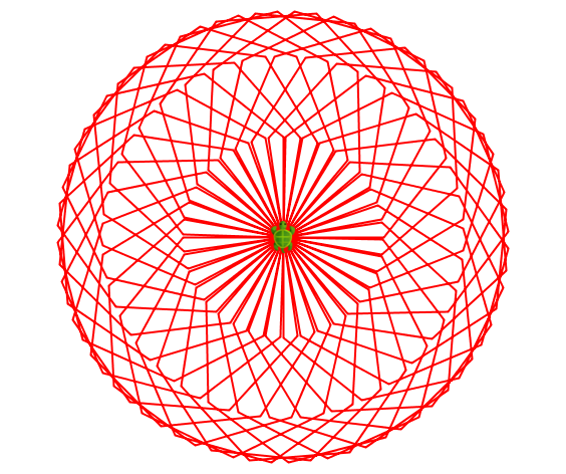
\includegraphics[width=12.0cm]{../img/polygons-circle.png}};
\end{tikzpicture}
  

\begin{lstlisting}[basicstyle={\ttfamily\fontsize{16}{19}\selectfont},numbers=none]
def polygon(n: Heltal, sidlängd: Heltal) = upprepa(n){
  fram(sidlängd)
  vänster(360.0/n)
}
def snurra(n: Heltal, vinkel: Heltal, sidlängd: Heltal) = 
  upprepa(360/vinkel){ polygon(n, sidlängd); vänster(vinkel) }

sudda; sakta(5)
snurra(7, 10, 100)
\end{lstlisting}
        
\chapter{Slumptal}\section*{\color{BrickRed}Uppdrag:}


\begin{itemize}

\item {Kör programmet nedan många gånger. Vad händer?}
\item {Vilket är det minsta och största möjliga värdet på radien \lstinline{r}?}
\item {Ändra så att \lstinline{r} blir ett slumptal mellan 3 och 200.}
\item {Rita 100 cirklar med slumpmässig radie på slumpmässig plats, som bilden visar.}

\end{itemize}



\begin{tikzpicture}[overlay]
\node at (21.0cm,-5.0cm) {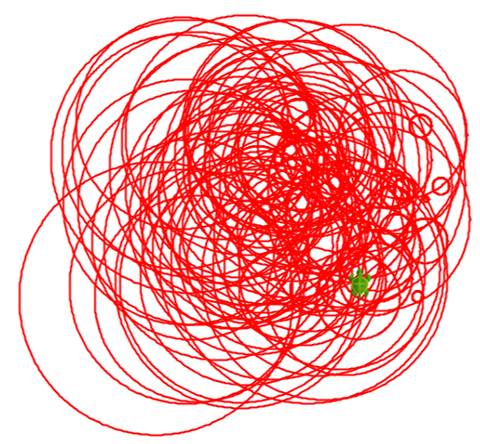
\includegraphics[width=8.0cm]{../img/random-circles.png}};
\end{tikzpicture}
  

\begin{lstlisting}[basicstyle={\ttfamily\fontsize{20}{24}\selectfont},numbers=none]
//värdet r blir ett slumptal mellan 10 och 89:
val r = slumptal(90) + 10   

sudda; sakta(10); osynlig
skriv("Radie = " + r)
cirkel(r)
\end{lstlisting}
        
\chapter{Blanda dina egna färger}

\begin{itemize}

\item {Med \lstinline{Color} kan du blanda egna färger, till exempel \lstinline{Color(0, 70, 0)}}
\item {De tre parametrarna anger mängden {\it rött}, {\it grönt} och {\it blått}}
\item {Du kan också lägga till en fjärde parameter som anger {\it genomskinligheten}}
\item {Alla parametrar ska vara mellan 0 och 255}

\end{itemize}


\section*{\color{BrickRed}Uppdrag:}
Prova programmet nedan. Ändra genomskinligheten.

\begin{tikzpicture}[overlay]
\node at (23.0cm,-2.0cm) {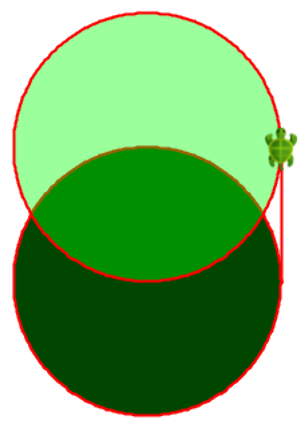
\includegraphics[width=7.0cm]{../img/color-circles.png}};
\end{tikzpicture}
  

\begin{lstlisting}[basicstyle={\ttfamily\fontsize{16}{19}\selectfont},numbers=none]
sudda; sakta(100)      

val olivgrön = Color(0,70,0)
val pistageglass = Color(0,255,0,100)

fyll(olivgrön); cirkel(100)
fyll(pistageglass); fram(100); cirkel(100)
\end{lstlisting}
        
\chapter{Prova färgväljaren}
\begin{multicols}{2}
\section*{\color{BrickRed}Uppdrag:}


\begin{itemize}

\item {Högerklicka i editor-fönstret och klicka på "Välj färg".}
\item {Om du väljer fliken {\bf RGB} i färgväljaren kan du blanda nya RGB-färger.}
\item {Tryck OK och titta i Utdatafönstret. Där syns de tre RGB-värdena för rött, grönt och blått.}
\item {Du kan använda dessa värden i ditt program för att rita med din nya färg med \lstinline{färg(Color(218, 153, 67))}.}

\end{itemize}



\columnbreak

\begin{center}
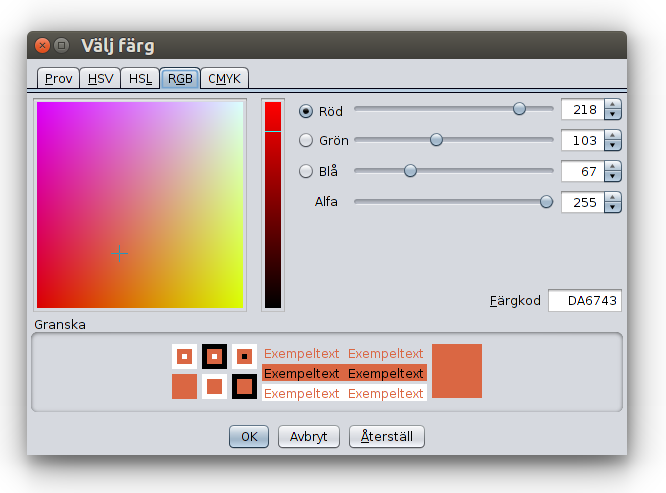
\includegraphics[width=14.0cm]{../img/color-chooser-rgb-sv.png}
\end{center}

\end{multicols}

\chapter{Rita slumpcirklar}
\begin{multicols}{2}

\begin{lstlisting}[basicstyle={\ttfamily\fontsize{16}{19}\selectfont},numbers=none]
def slump = slumptal(256)
def slumpfärg = Color(slump,10,slump,100) 

sudda; sakta(5)
bakgrund2(svart,vit)
bredd(6)

upprepa(100) {
    färg(slumpfärg)
    cirkel(100)
    hoppa(20)
    höger(35)
}
\end{lstlisting}
        
\section*{\color{BrickRed}Uppdrag:}
Prova olika slumpfärger och bakgrunder.


\columnbreak


\begin{center}
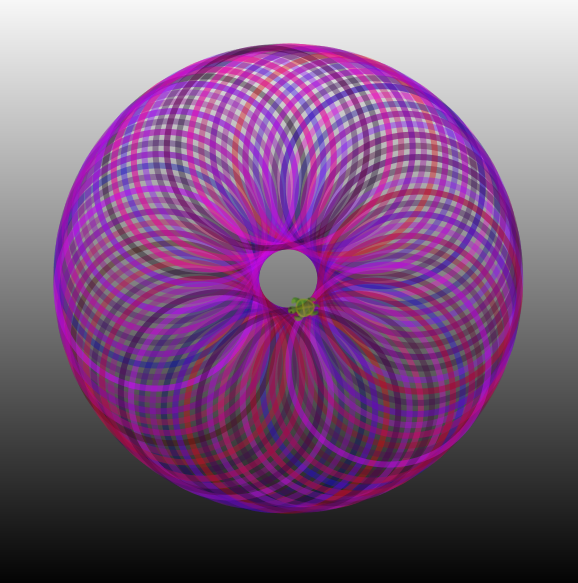
\includegraphics[width=12.0cm]{../img/circle-of-circles.png}
\end{center}

\end{multicols}

\chapter{Rita en blomma}\section*{\color{BrickRed}Uppdrag:}
Programmet nedan ritar 100 slumpfärgade cirklar på slumpmässig plats med slumpmässig radie. Prova att ändra de olika slumptalens gränser och försök förklara vad som händer.

\begin{tikzpicture}[overlay]
\node at (21.5cm,-4.0cm) {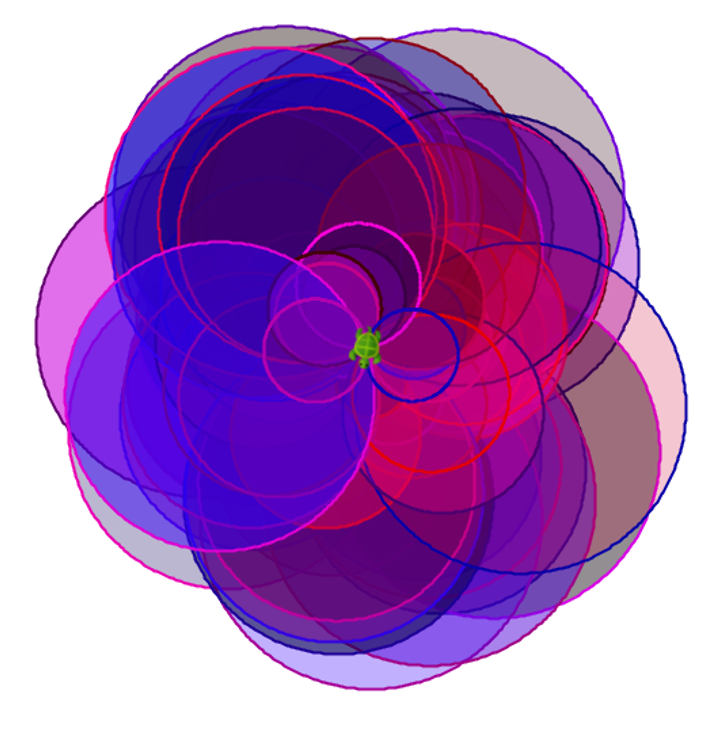
\includegraphics[width=9.0cm]{../img/random-color-circles.png}};
\end{tikzpicture}
  

\begin{lstlisting}[basicstyle={\ttfamily\fontsize{16}{19}\selectfont},numbers=none]
sudda(); sakta(5)
bredd(2)
upprepa(100){
  färg(Color(slumptal(256),0,slumptal(256)))
  fyll(Color(slumptal(256),0,slumptal(256),slumptal(100)+50))
  vänster(slumptal(360))
  cirkel(slumptal(30)*4+10)
}
\end{lstlisting}
        
\chapter{Rita många blommor}\section*{\color{BrickRed}Uppdrag:}


\begin{itemize}

\item {Gör en funktion som heter \lstinline{blomma}, som ritar en krona och en grön stjälk från kronans mitt med ett grönt blad.}
\item {Rita 5 blommor bredvid varandra.}

\end{itemize}



\begin{tikzpicture}[overlay]
\node at (15.0cm,-7.0cm) {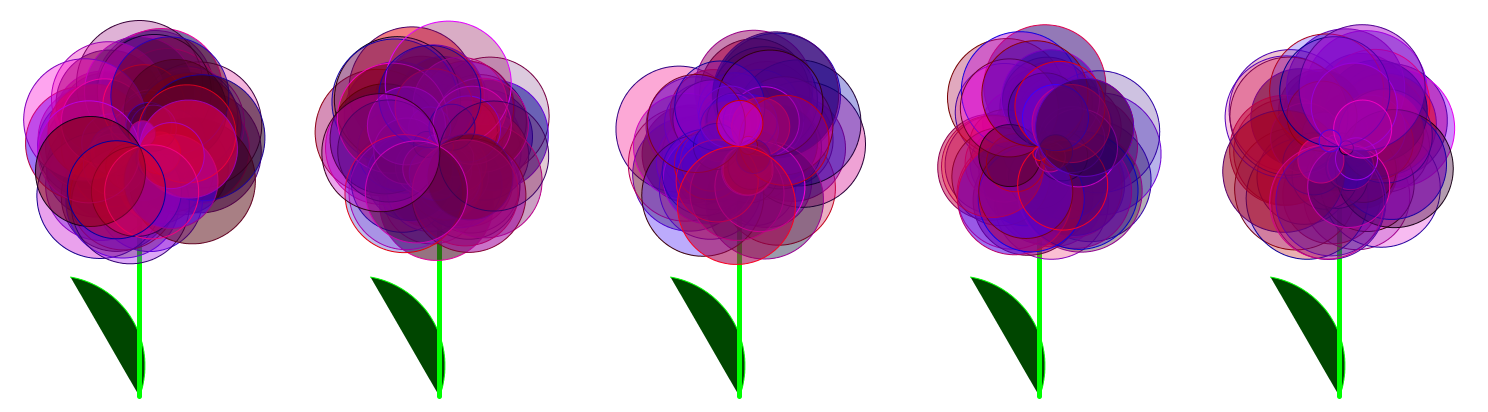
\includegraphics[width=16.0cm]{../img/flowers.png}};
\end{tikzpicture}
  
\section*{\color{OliveGreen}Tips:}
Du kan rita blad med \lstinline{båge(radie, vinkel)}. \\
Låt funktionen \lstinline{blomma} ha två parametrar x och y och använd \lstinline{hoppaTill(x,y)}\\
Du kan loopa 5 gånger och räkna ut platsen så här:

\begin{lstlisting}[basicstyle={\ttfamily\fontsize{18}{22}\selectfont},numbers=none]
var i = 0          
upprepa(5){
  blomma(600*i,0)
  i = i + 1        
}
\end{lstlisting}
        
\chapter{Hur snabb är din dator?}I Kojo finns en funktion \lstinline{räknaTill} som mäter hur snabbt datorn kan räkna.\\
När jag kör \lstinline{räknaTill(5000)} på min snabba dator skrivs detta i utdata-fönstret:

\begin{lstlisting}[numbers=none]

*** Räknar från 1 till ... 5000 *** KLAR!
Det tog 0.32 millisekunder.
      
\end{lstlisting}
        
\section*{\color{BrickRed}Uppdrag:}


\begin{itemize}

\item {Kör \lstinline{räknaTill(5000)} och kolla om din dator är snabbare än min.}
\item {Hur lång tid tar det för din dator att räkna till en miljon?}
\item {Hur långt hinner din dator räkna till på en sekund?}

\end{itemize}


\chapter{Byt kostym på paddan}\section*{\color{BrickRed}Uppdrag:}
Ladda ner mediafiler från Kojos hemsida:
\href{http://www.kogics.net/kojo-download#media}{www.kogics.net/kojo-download\#media}
\\

Skapa en mapp \lstinline{Kojo} i din hemkatalog om det inte redan finns en sådan.\\
Packa upp filen \lstinline{scratch-media.zip} och lägg mappen Media i mappen Kojo.\\
Prova att byta kostym på paddan till en häst så här:

\begin{tikzpicture}[overlay]
\node at (22.0cm,-2.5cm) {
\includegraphics{../img/horse1-a.png}};
\end{tikzpicture}
  

\begin{lstlisting}[basicstyle={\ttfamily\fontsize{20}{24}\selectfont},numbers=none]
sudda
kostym("~/Kojo/Media/Costumes/Animals/horse1-a.png")
sakta(2000)
fram(1000)
\end{lstlisting}
        
\section*{\color{OliveGreen}Tips:}
Du kan också använda dina egna bilder av typen \lstinline{.png} eller \lstinline{.jpg}
\chapter{Gör en timer}\section*{\color{BrickRed}Uppdrag:}
Prova programmet nedan och mät din reaktionstid. Hur snabb är du?

\begin{lstlisting}[basicstyle={\ttfamily\fontsize{18}{22}\selectfont},numbers=none]
object timer {
  def nu = System.currentTimeMillis  //ger nutid i millisekunder
  var tid = nu
  def nollställ = { tid = nu }
  def mät = nu - tid
  def slumpvänta(min: Int, max: Int) =  //vänta mellan min och max sekunder
    Thread.sleep((slumptal(max-min)+min)*1000)  //Thread.sleep(1000) väntar 1 sekund
}

utdata("Klicka i utdatafönstret och vänta...")
timer.slumpvänta(3,6)   //vänta mellan 3 och 6 sekunder
timer.nollställ
indata("Tryck Enter så snabbt du kan.")
utdata("Reaktionstid: " + (timer.mät/1000.0) + " sekunder")
\end{lstlisting}
        
\chapter{Träna multiplikation}\section*{\color{BrickRed}Uppdrag:}
Prova programmet nedan. Ändra så att man bara tränar 8:ans och 9:ans tabell.

\begin{lstlisting}[basicstyle={\ttfamily\fontsize{16}{19}\selectfont},numbers=none]
var antalRätt = 0
val startTid = System.currentTimeMillis / 1000
upprepa(12) {
  val tal1 = slumptal(12)+1
  val tal2 = slumptal(12)+1
  val svar = indata("Vad är " + tal1 + "*" + tal2 + "?")
  if (svar == (tal1 * tal2).toString) {
    utdata("Rätt!")
    antalRätt = antalRätt + 1
  }
  else utdata("Fel. Rätt svar är " + (tal1 * tal2))
}
val stoppTid = System.currentTimeMillis / 1000
val sek = stoppTid - startTid
utdata("Du fick " + antalRätt + " rätt på " + sek + " sekunder.")
\end{lstlisting}
        
\chapter{Spara saker i en vektor}\section*{\color{BrickRed}Uppdrag:}
Prova programmet nedan. Vad skrivs ut? Lägg till fler djur i vektorn.

\begin{lstlisting}[basicstyle={\ttfamily\fontsize{16}{19}\selectfont},numbers=none]
var djur = Vector("älg", "ko", "kanin", "kvalster")
utdata("Första djuret i listan är: " + djur(0))  //platserna i vektorn räknas från 0
utdata("Andra djuret i listan är:  " + djur(1))
utdata("Det finns så här många djur: " + djur.size)
utdata("Sista djuret i listan är:  " + djur(djur.size-1))

val s = slumptal(djur.size)   //dra ett slumpal mellan 0 och antalet djur minus 1
utdata("Ett slumpmässigt djur: " + djur(s))

djur = djur :+ "Kamel" //lägg till ett djur sist i vektorn
djur = djur.updated(0, "Dromedar")  //Ändra djuret på plats 0
utdata("Alla djur i vektorn baklänges:")
djur.foreach{x => utdata(x.reverse)} //för alla x i vektorn: skriv ut x baklänges
\end{lstlisting}
        
\chapter{Simulera ett trafikljus}\section*{\color{BrickRed}Uppdrag:}
Prova programmet nedan. Ändra så att trafikljuset är rött dubbelt så länge.

\begin{tikzpicture}[overlay]
\node at (22.0cm,-6.0cm) {
\includegraphics[width=3.0cm]{../img/traffic-lights.png}};
\end{tikzpicture}
  

\begin{lstlisting}[basicstyle={\ttfamily\fontsize{14}{17}\selectfont},numbers=none]
def släckAlla = draw(penColor(gray) * fillColor(black) -> PicShape.rect(130,40))
def ljus(c: Color, h: Int) = penColor(noColor) * fillColor(c) * trans(20,h) -> PicShape.circle(15)
def rött = draw(ljus(red, 100))
def gult = draw(ljus(yellow, 65))
def grönt = draw(ljus(green, 30))
def vänta(sekunder: Int) = Thread.sleep(sekunder*1000)

clear; invisible  
while (true) { //en oändlig loop
  släckAlla
  rött;  vänta(3)
  gult;  vänta(1) 
  släckAlla
  grönt; vänta(3)
  gult;  vänta(1)
}
\end{lstlisting}
        
